\documentclass[11pt]{article}
\usepackage{certmachine}
%% generated by tools/paper-numbers/mfg-redecided.js from certs/agtable-redecided.json, certs/afg-enclosure.json, certs/hbar-band.json, certs/maxval-cylinder.json, certs/regatlas.json, certs/price-band.json, certs/aag-empty-region.json and the re-run Wardrop verifier — do not edit (git eece01c1497a)
\newcommand{\RepoCommit}{eece01c1497a}
\newcommand{\AGCells}{24}
\newcommand{\AGReproduced}{13}
\newcommand{\AGNear}{5}
\newcommand{\AGDiffers}{6}
\newcommand{\AGTestOneRep}{4}
\newcommand{\AGTestOneNear}{3}
\newcommand{\AGTestOneDiff}{5}
\newcommand{\AGTestTwoRep}{9}
\newcommand{\AGTestTwoNear}{2}
\newcommand{\AGTestTwoDiff}{1}
\newcommand{\AGEpsOne}{0.004}
\newcommand{\AGEpsTwo}{0.0002}
\newcommand{\AGTight}{$1\times10^{-8}$}
\newcommand{\AGMeshes}{(100, 25), (200, 50), (400, 100), (800, 200)}
\newcommand{\AGLamOne}{1.1}
\newcommand{\AGLamTwo}{1.2}
\newcommand{\AGTolShare}{39}
\newcommand{\AGFinestPrintedW}{$2.1\times10^{-3}$}
\newcommand{\AGFinestTheirsW}{$2.07\times10^{-3}$}
\newcommand{\AGFinestTightW}{$1.49\times10^{-3}$}
\newcommand{\AGIterTheirs}{4}
\newcommand{\AGIterTight}{14--15}
\newcommand{\AGIterTwo}{3}
\newcommand{\AGResidTwo}{$5.5\times10^{-13}$}
\newcommand{\AGOrdersW}{2.04, 2.02, 2.01}
\newcommand{\AGPrintedRatiosW}{2.00, 1.82, 1.57}
\newcommand{\AGOrdersWTwo}{2.00, 2.00, 2.00}
\newcommand{\AGaZeroBox}{[-0.029123125, -0.029123055]}
\newcommand{\AGaZeroRem}{$6.9\times10^{-8}$}
\newcommand{\AGaZeroK}{4{,}096}
\newcommand{\AGKOneBox}{[0.02810377506, 0.02810377507]}
\newcommand{\AGQOneBox}{[0.44861785366, 0.44861785367]}
\newcommand{\AGSigmaT}{0.648054}
\newcommand{\AGMassOneBox}{[0.403630, 0.403631]}
\newcommand{\AGMassTwoBox}{[0.369994, 0.369995]}
\newcommand{\AGIntTwoBox}{[0.05588298, 0.05588337]}
\newcommand{\AGPriceWidthOne}{$1.5\times10^{-14}$}
\newcommand{\AGPriceWidthTwo}{$1.2\times10^{-13}$}
\newcommand{\AGClearingHalf}{$1.3\times10^{-14}$}
\newcommand{\AGGridN}{200}
\newcommand{\AGMaxErrWidth}{$3.6\times10^{-7}$}
\newcommand{\AGSliverFrom}{0.9101}
\newcommand{\AGSliverTo}{0.9111}
\newcommand{\AGSliverTwoFrom}{0.8343}
\newcommand{\AGSliverTwoTo}{0.8353}
\newcommand{\AGExponentAtTo}{227}
\newcommand{\AGMassOne}{$3.9\times10^{95}$}
\newcommand{\AGMassTwo}{$2.3\times10^{87}$}
\newcommand{\AGuFactorFinest}{2.36}
\newcommand{\AGmFactorFinest}{1.58}
\newcommand{\AGwTwoFinestFactor}{0.85}
\newcommand{\AGRowsOne}{0.0200 & $\varpi$ & $1.2\times10^{-2}$ & $1.23\times10^{-2}$ & $1.23\times10^{-2}$ & \textsc{reproduced} \\
 & $u(\cdot,0)$ & $2.5\times10^{-2}$ & $2.67\times10^{-2}$ & $2.72\times10^{-2}$ & \textsc{near} ($\times$1.07) \\
 & $m(\cdot,T)$ & $8.8\times10^{-2}$ & $9.31\times10^{-2}$ & $9.49\times10^{-2}$ & \textsc{near} ($\times$1.06) \\
\addlinespace[2pt] 0.0100 & $\varpi$ & $6.0\times10^{-3}$ & $6.04\times10^{-3}$ & $6.04\times10^{-3}$ & \textsc{reproduced} \\
 & $u(\cdot,0)$ & $1.1\times10^{-2}$ & $1.32\times10^{-2}$ & $1.38\times10^{-2}$ & \textsc{differs} ($\times$1.20) \\
 & $m(\cdot,T)$ & $4.2\times10^{-2}$ & $4.69\times10^{-2}$ & $4.88\times10^{-2}$ & \textsc{near} ($\times$1.12) \\
\addlinespace[2pt] 0.0050 & $\varpi$ & $3.3\times10^{-3}$ & $3.27\times10^{-3}$ & $2.99\times10^{-3}$ & \textsc{reproduced} \\
 & $u(\cdot,0)$ & $4.7\times10^{-3}$ & $6.31\times10^{-3}$ & $6.96\times10^{-3}$ & \textsc{differs} ($\times$1.34) \\
 & $m(\cdot,T)$ & $1.8\times10^{-2}$ & $2.28\times10^{-2}$ & $2.48\times10^{-2}$ & \textsc{differs} ($\times$1.27) \\
\addlinespace[2pt] 0.0025 & $\varpi$ & $2.1\times10^{-3}$ & $2.07\times10^{-3}$ & $1.49\times10^{-3}$ & \textsc{reproduced} \\
 & $u(\cdot,0)$ & $1.2\times10^{-3}$ & $2.83\times10^{-3}$ & $3.49\times10^{-3}$ & \textsc{differs} ($\times$2.36) \\
 & $m(\cdot,T)$ & $6.7\times10^{-3}$ & $1.06\times10^{-2}$ & $1.25\times10^{-2}$ & \textsc{differs} ($\times$1.58) \\}
\newcommand{\AGRowsTwo}{0.0200 & $\varpi$ & $2.6\times10^{-2}$ & $2.66\times10^{-2}$ & $2.66\times10^{-2}$ & \textsc{near} ($\times$1.02) \\
 & $u(\cdot,0)$ & $8.5\times10^{-3}$ & $8.53\times10^{-3}$ & $8.53\times10^{-3}$ & \textsc{reproduced} \\
 & $m(\cdot,T)$ & $5.3\times10^{-2}$ & $5.27\times10^{-2}$ & $5.27\times10^{-2}$ & \textsc{reproduced} \\
\addlinespace[2pt] 0.0100 & $\varpi$ & $1.3\times10^{-2}$ & $1.33\times10^{-2}$ & $1.33\times10^{-2}$ & \textsc{reproduced} \\
 & $u(\cdot,0)$ & $7.4\times10^{-3}$ & $7.38\times10^{-3}$ & $7.38\times10^{-3}$ & \textsc{reproduced} \\
 & $m(\cdot,T)$ & $2.6\times10^{-2}$ & $2.64\times10^{-2}$ & $2.64\times10^{-2}$ & \textsc{reproduced} \\
\addlinespace[2pt] 0.0050 & $\varpi$ & $6.7\times10^{-3}$ & $6.63\times10^{-3}$ & $6.63\times10^{-3}$ & \textsc{near} ($\times$0.99) \\
 & $u(\cdot,0)$ & $6.8\times10^{-3}$ & $6.78\times10^{-3}$ & $6.78\times10^{-3}$ & \textsc{reproduced} \\
 & $m(\cdot,T)$ & $1.3\times10^{-2}$ & $1.32\times10^{-2}$ & $1.32\times10^{-2}$ & \textsc{reproduced} \\
\addlinespace[2pt] 0.0025 & $\varpi$ & $3.9\times10^{-3}$ & $3.32\times10^{-3}$ & $3.32\times10^{-3}$ & \textsc{differs} ($\times$0.85) \\
 & $u(\cdot,0)$ & $6.5\times10^{-3}$ & $6.45\times10^{-3}$ & $6.45\times10^{-3}$ & \textsc{reproduced} \\
 & $m(\cdot,T)$ & $6.6\times10^{-3}$ & $6.62\times10^{-3}$ & $6.62\times10^{-3}$ & \textsc{reproduced} \\}
\newcommand{\AFGjBox}{[0.3461135133, 0.3461135308]}
\newcommand{\AFGHBox}{[0.1711645502, 0.1711645817]}
\newcommand{\AFGjHalf}{$8.7\times10^{-9}$}
\newcommand{\AFGHHalf}{$1.6\times10^{-8}$}
\newcommand{\AFGmMin}{0.4291}
\newcommand{\AFGmMax}{2.3164}
\newcommand{\AFGCtrlHBox}{[0.2359143495, 0.2359143676]}
\newcommand{\AFGCtrlHHalf}{$9.0\times10^{-9}$}
\newcommand{\AFGCtrlCFBox}{[0.2359143540, 0.2359143631]}
\newcommand{\AFGCtrlCFHalf}{$4.5\times10^{-9}$}
\newcommand{\AFGCtrljHalf}{$1.0\times10^{-13}$}
\newcommand{\AFGCtrlmMin}{0.2905}
\newcommand{\AFGCtrlmMax}{2.1471}
\newcommand{\AFGIntExpVBox}{[1.26606587, 1.26606589]}
\newcommand{\AFGKF}{16{,}384}
\newcommand{\AFGKD}{2{,}048}
\newcommand{\AFGKP}{256}
\newcommand{\AFGRounds}{1}
\newcommand{\AFGClosureHalf}{$2.9\times10^{-8}$}
\newcommand{\AFGFalsifiers}{5}
\newcommand{\AFGuAmp}{0.0775}
\newcommand{\HBSampled}{22}
\newcommand{\HBFlat}{9}
\newcommand{\HBRotating}{12}
\newcommand{\HBUndecided}{1}
\newcommand{\HBPZeroBox}{[1.273238818, 1.273240334]}
\newcommand{\HBPZeroWidth}{$1.5\times10^{-6}$}
\newcommand{\HBFourOverPi}{1.273239545}
\newcommand{\HBWidthMin}{$1.5\times10^{-6}$}
\newcommand{\HBWidthMax}{$2.0\times10^{-6}$}
\newcommand{\HBWidestP}{3}
\newcommand{\HBRotFirstP}{1.275}
\newcommand{\HBRotLastP}{3}
\newcommand{\HBKSweep}{1{,}024}
\newcommand{\HBKTable}{8{,}192}
\newcommand{\HBKPZero}{4{,}096}
\newcommand{\HBTableOneBox}{[4.409965233, 4.409965294]}
\newcommand{\HBTableOneWidth}{$6.0\times10^{-8}$}
\newcommand{\HBTableOneMid}{4.4099653}
\newcommand{\HBCFifteenBox}{[1.244637626, 1.244637656]}
\newcommand{\HBCTwoFiveBox}{[3.165327607, 3.165327639]}
\newcommand{\HBCited}{4.4099660}
\newcommand{\HBCitedGap}{$7.1\times10^{-7}$}
\newcommand{\HBTableOneKs}{10, 100, 1{,}000, 10{,}000}
\newcommand{\HBTableOneLastNM}{4.40996}
\newcommand{\HBTableOneRows}{10 & 4.40251 & \textsc{below} & 4.40935 & \textsc{below} \\
100 & 4.40916 & \textsc{below} & 4.40994 & \textsc{below} \\
1{,}000 & 4.40989 & \textsc{below} & 4.40996 & \textsc{below} \\
10{,}000 & 4.40996 & \textsc{below} & 4.40996 & \textsc{below} \\}
\newcommand{\HBTableTwoK}{100}
\newcommand{\HBTableTwoP}{0.5}
\newcommand{\HBTableTwoRows}{15 & 0.964609 & 1 (\textsc{flat}, decided) & 0.03539 \\
30 & 0.964754 & 1 (\textsc{flat}, decided) & 0.03525 \\
60 & 0.964760 & 1 (\textsc{flat}, decided) & 0.03524 \\
120 & 0.964760 & 1 (\textsc{flat}, decided) & 0.03524 \\}
\newcommand{\HBTableTwoGapMin}{0.0352}
\newcommand{\HBTableTwoGapMax}{0.0354}
\newcommand{\HBPeriodTwoBox}{[0.5172097, 0.5172102]}
\newcommand{\MVCells}{3{,}072}
\newcommand{\MVSupport}{1{,}842}
\newcommand{\MVDecided}{1{,}150}
\newcommand{\MVRefused}{80}
\newcommand{\MVTight}{388}
\newcommand{\MVBracket}{762}
\newcommand{\MVGapProven}{786}
\newcommand{\MVGapShare}{68}
\newcommand{\MVMaxGap}{0.731}
\newcommand{\MVNT}{32}
\newcommand{\MVNX}{96}
\newcommand{\MVT}{1.5621}
\newcommand{\MVTHalf}{$4.4\times10^{-15}$}
\newcommand{\MVL}{6}
\newcommand{\MVrZero}{2}
\newcommand{\MVrT}{$\tfrac{3}{2}$}
\newcommand{\MVRhoZero}{$\tfrac{9}{4}$}
\newcommand{\MVFalsifiers}{5}
\newcommand{\RGCells}{50}
\newcommand{\RGProved}{34}
\newcommand{\RGRefused}{16}
\newcommand{\RGRefusedZOne}{15}
\newcommand{\RGRefusedNear}{1}
\newcommand{\RGAmpsList}{0, 0.1, 0.2, 0.3, 0.4, 0.5, 0.6, 0.7, 0.8, 0.9}
\newcommand{\RGEpsList}{0, 0.01, 0.1, 0.3, 1}
\newcommand{\RGNu}{1.05}
\newcommand{\RGNMin}{24}
\newcommand{\RGNMax}{40}
\newcommand{\RGrMin}{$9\times10^{-16}$}
\newcommand{\RGrMax}{$7\times10^{-8}$}
\newcommand{\RGFrontierRows}{0 & 0.7 & 0.8 & 1.219 & 0.320 & 0.225 \\
0.01 & 0.7 & 0.8 & 1.244 & 0.311 & 0.216 \\
0.1 & 0.6 & 0.7 & 1.089 & 0.341 & 0.245 \\
0.3 & 0.5 & 0.6 & 0.997 & 0.346 & 0.251 \\
1 & 0.4 & 0.5 & 1.030 & 0.299 & 0.204 \\}
\newcommand{\RGEpsZeroLast}{0.7}
\newcommand{\RGEpsLast}{1}
\newcommand{\RGEpsLastLast}{0.4}
\newcommand{\RGDistDecided}{26}
\newcommand{\RGDistMaxWidth}{$2.0\times10^{-7}$}
\newcommand{\RGDistHead}{$\varepsilon = 0.01$ & $\varepsilon = 0.1$ & $\varepsilon = 0.3$ & $\varepsilon = 1$}
\newcommand{\RGDistRows}{0 & 0.00971 & 0.07830 & 0.17095 & 0.31767 \\
0.1 & 0.00982 & 0.07919 & 0.17308 & 0.32231 \\
0.2 & 0.00995 & 0.08039 & 0.17602 & 0.32900 \\
0.3 & 0.01015 & 0.08211 & 0.18034 & 0.33950 \\
0.4 & 0.01043 & 0.08472 & 0.18719 & 0.35779 \\
0.5 & 0.01090 & 0.08905 & 0.19914 & --- \\
0.6 & 0.01171 & 0.09702 & --- & --- \\
0.7 & 0.01337 & --- & --- & --- \\
0.8 & --- & --- & --- & --- \\
0.9 & --- & --- & --- & --- \\}
\newcommand{\RGRatiosAFour}{1.04, 0.85, 0.62, 0.36}
\newcommand{\RGuOneAtZero}{0.6823}
\newcommand{\RGDistZeroOne}{0.3177}
\newcommand{\RGFloorLastZero}{0.320}
\newcommand{\RGFloatFirstZero}{0.225}
\newcommand{\RGZOneFirstZero}{1.22}
\newcommand{\RGZOneRowZero}{0.10, 0.21, 0.32, 0.44, 0.58, 0.74, 0.94, 1.22, 1.64}
\newcommand{\WDBoxRadius}{$7.32\times10^{-13}$}
\newcommand{\WDErratumFrac}{$\tfrac{1940}{37}$}
\newcommand{\WDErratumValue}{52.432}
\newcommand{\WDErratumRounds}{52}
\newcommand{\WDPrinted}{54}
\newcommand{\WDMaxDevFrac}{$\tfrac{58}{37}$}
\newcommand{\WDMaxDev}{1.568}
\newcommand{\WDNullDim}{6}
\newcommand{\WDUnknowns}{38}
\newcommand{\WDNodes}{10}
\newcommand{\WDEdges}{15}
\newcommand{\WDFlowFloor}{2.6205}
\newcommand{\WDSlackFloor}{0.3301}
\newcommand{\WDReds}{6}
\newcommand{\WDVerifierSha}{5d5fca032ff5dbb7}
\newcommand{\WDVerifierKB}{44}
\newcommand{\PRTheta}{-1.656370}
\newcommand{\PRThetaExact}{$-\tfrac{298385140072281459}{180143985094819840}$}
\newcommand{\PREnergy}{0.686096}
\newcommand{\PRXiT}{0.988031}
\newcommand{\PRxBar}{0.301935}
\newcommand{\PRc}{1}
\newcommand{\PRGamma}{12}
\newcommand{\PRZeta}{$\tfrac{17}{20}$}
\newcommand{\PRN}{240}
\newcommand{\PRGridTimes}{241}
\newcommand{\PRRhoPct}{15}
\newcommand{\PRRhoFrac}{$\tfrac{3}{20}$}
\newcommand{\PRWidest}{2.7747}
\newcommand{\PRWidestHour}{12}
\newcommand{\PRWidestExact}{$\tfrac{4998384929455593201}{1801439850948198400}$}
\newcommand{\PRDayPart}{2.4699}
\newcommand{\PRInstAtWidest}{0.3047}
\newcommand{\PRInstMax}{0.305}
\newcommand{\PRDayShare}{89}
\newcommand{\PRRhoForOne}{5.41}
\newcommand{\PRWidthAtZero}{2.5965}
\newcommand{\PRPiZero}{1.6564}
\newcommand{\PRPiT}{1.6564}
\newcommand{\PRLadderRows}{0 & 0 & 2.7747 & 12 & 0.305 & 2.470 & 0.000 & 1.6564 & 1.6564 \\
3 & $\tfrac{3}{5}$ & 3.0235 & 11 & 0.297 & 2.470 & 0.256 & 1.7539 & 1.6564 \\
12 & $\tfrac{3}{5}$ & 3.8292 & 8 & 0.251 & 2.470 & 1.108 & 2.0466 & 1.6564 \\}
\newcommand{\PRFalsifiers}{5}
\newcommand{\PREnergyLo}{0.5832}
\newcommand{\PREnergyHi}{0.7890}
\newcommand{\PRKernelRows}{lab walls, control-cleared & 0.9032 & 0.0848 & 0.039 & 22.9 & 49 & $8.0\times10^{-10}$ \\
constraint walls, control-cleared & 0.9235 & 0.0645 & 0.566 & 8.1 & 36 & $9.8\times10^{-10}$ \\
constraint walls, flux-cleared & 0.9880 & $1\times10^{-14}$ & 1.280 & 70.5 & 52 & $8.6\times10^{-10}$ \\}
\newcommand{\PRLabXiT}{0.9032}
\newcommand{\PRLabLost}{0.0848}
\newcommand{\PRLabLostPct}{12.4}
\newcommand{\PRConstrainedLost}{0.0645}
\newcommand{\PRConsistentLost}{$1\times10^{-14}$}
\newcommand{\PRLabClearGap}{$8.9\times10^{-16}$}
\newcommand{\PRLabIt}{49}
\newcommand{\PRLabRes}{$8.0\times10^{-10}$}
\newcommand{\PRLabNX}{120}
\newcommand{\PRLabNT}{240}
\newcommand{\PRWallDensityLab}{22.9}
\newcommand{\PRShadow}{0.376}
\newcommand{\PRLabPiMid}{0.039}
\newcommand{\PRConsistentPiMid}{1.280}
\newcommand{\PROrder}{1.88}
\newcommand{\PRLabOrder}{0.72}
\newcommand{\PRWideA}{-1}
\newcommand{\PRWideB}{2}
\newcommand{\PRWideRows}{flux-cleared, constrained walls & 0.0201 & 150 $\times$ 240 & 0.0816 \\
 & 0.0100 & 300 $\times$ 480 & 0.0434 \\
the lab's walls, control-cleared & 0.0201 & 150 $\times$ 240 & 1.6998 \\
 & 0.0100 & 300 $\times$ 480 & 2.3615 \\}
\newcommand{\PRWideEtaErr}{0.0882}
\newcommand{\PRWideEta}{6}
\newcommand{\PRWideErrCoarse}{0.0816}
\newcommand{\PRWideErrFine}{0.0434}
\newcommand{\PRLabWideErrCoarse}{1.6998}
\newcommand{\PRLabWideErrFine}{2.3615}
\newcommand{\AAGK}{256}
\newcommand{\AAGRefused}{4}
\newcommand{\AAGRefusedLength}{0.015625}
\newcommand{\AAGLadderKs}{16, 64, 256, 1024}
\newcommand{\AAGLadderFirstLength}{0.25}
\newcommand{\AAGLadderLastLength}{0.00390625}
\newcommand{\AAGLadderLastK}{1{,}024}
\newcommand{\AAGRunsRows}{$[0.00000,\ 0.08203)$ & \textsc{occupied} & $m = V$, enclosed on each cell \\
$[0.08203,\ 0.08594)$ & \textsc{refused} & holds a root of $V$ at this budget \\
$[0.08594,\ 0.41406)$ & \textsc{empty} & $m = 0$ exactly \\
$[0.41406,\ 0.41797)$ & \textsc{refused} & holds a root of $V$ at this budget \\
$[0.41797,\ 0.74609)$ & \textsc{occupied} & $m = V$, enclosed on each cell \\
$[0.74609,\ 0.75391)$ & \textsc{refused} & holds a root of $V$ at this budget \\
$[0.75391,\ 1.00000)$ & \textsc{empty} & $m = 0$ exactly \\}
\newcommand{\AAGEmptyRuns}{2}
\newcommand{\AAGOccupiedRuns}{2}
\newcommand{\AAGuPlusZeroBox}{[0.4540, 0.4664]}
\newcommand{\AAGuGapZero}{0.908}
\newcommand{\AAGGammaBox}{[-0.5, -0.3]}
\newcommand{\AAGCaseTwoFloor}{0.0684}
\newcommand{\AAGCaseTwoMax}{0.2691}
\newcommand{\AAGjZero}{$\tfrac{1}{10}$}
\newcommand{\AAGVOneBox}{[-0.3536, -0.3535]}
\newcommand{\AAGmZeroBox}{[0.3535, 0.3536]}
\newcommand{\AAGExitFluxTwoBox}{[-0.1001, -0.0999]}
\newcommand{\AAGFalsifiers}{5}


\title{Published mean-field-game numerics, re-decided:\\
error tables, closed forms, effective Hamiltonians, value functions,\\
regularizations and prices as certified objects}
\author{\cmauthor}
\date{October 2026 --- draft v0.1 for review; every number interpolated from the record; machine-derived, not peer-reviewed; author list to be agreed}

\begin{document}
\maketitle

\begin{abstract}
Eight published pieces of mean-field-game numerics from one research line are taken back to the objects they print or define --- two convergence tables, a closed form used as a benchmark, an effective Hamiltonian with the values quoted for it, a maximal value function, a regularization sent to zero, a Wardrop equilibrium table, a clearing price and an empty region --- and each is met by an interval enclosure or an exact rational decision computed with no code shared with the authors. The verdicts are the words of the public records: a printed cell is \emph{reproduced} to its digits, \emph{near}, or \emph{differs} by a stated factor; a defined object is \emph{enclosed} to a stated width, \emph{proved} to exist in a box, or \emph{refused} by name. Of the \AGCells\ cells in the error tables of Ashrafyan and Gomes, \AGReproduced\ are reproduced to their two digits by a scheme written from the paper's description, \AGNear\ are within 15\% and \AGDiffers\ differ; two facts the tables could not show are found: the stopping tolerance is \AGTolShare\% of the finest printed price error, and the initial density as printed has no finite integral. A value quoted by Gomes and Yang for a separable effective Hamiltonian, \HBCited, lies \HBCitedGap\ above its enclosure; a Wardrop total printed as \WDPrinted\ is found to be \WDErratumFrac\ $= \WDErratumValue$. Every number here is interpolated from a record re-derived at every build of the repository.
\end{abstract}

\section{Introduction}\label{sec:intro}

A numerical paper ends with numbers: a table of errors against an exact solution, a value quoted from an earlier computation, a figure of an equilibrium found by a convergent flow. They are read as evidence that the method works, and they are trusted because the authors are. This note does the other thing for one research line, the mean-field-game numerics of Gomes and co-authors \cite{AG25,AFG17,GY20,GU26,FGU26,BAdHG26,GS21,AAG26}: it takes the printed numbers and the objects they are printed about and decides each one again with instruments that share no code with the authors --- outward-rounded interval arithmetic, exact rational arithmetic, and the two standard contraction arguments, Krawczyk's operator \cite{Kr69} and the radii polynomial \cite{vdBL15,DLM07}, with their side conditions checked in interval arithmetic. The outcome of a decision is a word from a short list (Section~\ref{sec:vocab}), and the word is a statement about an interval or an exact rational, never about a float.

What is new here is not any one enclosure --- the formulas enclosed are the papers' own or classical --- but the decision grammar applied uniformly to a body of published numerics, and the record: each verdict below is read from a JSON record in a public repository \cite{CM} that a build re-derives byte for byte before any page, or this document, can quote it (Section~\ref{sec:method}). A disagreement with a printed number is stated with its size and the choice it may rest on; nowhere is a theorem of the papers at issue (Section~\ref{sec:notclaimed}).

\section{Vocabulary}\label{sec:vocab}

The records use a fixed set of words, and so does this note.
\begin{description}
\item[Enclosed.] A quantity is enclosed when an interval computed in outward-rounded arithmetic (Section~\ref{sec:method}) is known to contain it; the width is always stated and carries every rounding and quadrature remainder.
\item[Decided.] A sign, an inclusion or an identity is decided when an enclosure or an exact computation settles it: a residual that encloses zero, a printed value above an enclosure, a cell on which a potential is positive. ``Found not to be'' is the phrase for a printed statement decided false.
\item[Proved.] An object is proved to exist, locally uniquely, when a contraction argument closes: a Krawczyk operator maps a box strictly into its interior, or a radii polynomial has a radius $r$ with $p(r) < 0$ and $\kappa = Z_1 + Z_2 r < 1$ --- both conditions, in interval arithmetic.
\item[Reproduced, near, differs.] For a printed error table: \textsc{reproduced} when the re-derived error, itself an interval, meets the rounding box of the printed digits (half a unit of the last printed digit on either side); \textsc{near} when it lies within 15\% of the printed value but outside the box; \textsc{differs} otherwise, with the factor between them --- a statement about an independent implementation of the described scheme, not about the printed number.
\item[Refused.] The arithmetic cannot decide at the budget it was given, or a contraction does not close ($Z_1 \ge 1$), and nothing is asserted about that cell or point; the reason is named, and the refusal is itself the verdict.
\item[Measured.] A floating-point computation at a fixed mesh, reported as such --- a scheme's error, a kernel's leak, a convergence ratio --- and never the authority for a decided number.
\item[Undecided, chosen.] A point inside the enclosure of a threshold is left undecided; a function that is one member of a set the data admits, such as a value function off the support of the density, is chosen and drawn as such.
\end{description}
We say an object is \emph{certified} when a statement about it has been decided or proved in this sense with the falsifiers of its certificate fired (Section~\ref{sec:method}); the word is used in no other sense.

\section{Two error tables (Ashrafyan--Gomes)}\label{sec:ag}

\paragraph{The published object.} Ashrafyan and Gomes \cite{AG25} discretize the price-formation game of \cite{GS21} by a fully discrete semi-Lagrangian scheme and end with two tables (\S8, Tables 1 and 2) of relative $\ell^\infty$ errors against ``semi-explicit'' solutions, at four meshes, $(M, N)$ equal to \AGMeshes, with $\rho = 2h$, to two significant digits, in three columns: the price $\varpi$ over the time grid, $u$ at $t = 0$ and $m$ at $t = T$ over the space grid. Both tests share the supply $\dot Q = 5\sin 3\pi t - 4Q$, $Q(0) = -\tfrac12$, $T = 1$, on $[-1, 1]$. Test 1 is linear-quadratic, $l_0 = \alpha^2/2$ and $V = (x - \tfrac14)^2/2$, with tolerance $\varepsilon = \AGEpsOne$; test 2 has $l_0 = \tfrac34|\alpha|^{4/3}$ and $V = x$, with $\varepsilon = \AGEpsTwo$. The initial density is printed as $\hat m(x) = \exp(-1/(1 - (\lambda x)^2))$ for $|x| < 1$, $\lambda = \AGLamOne$ and $\AGLamTwo$.

\paragraph{What was enclosed.} The two analytic solutions are evaluated as intervals: the supply and its integrals in closed form with $\pi$ and $e$ enclosed ($K(1) = \int_0^1 Q \in \AGKOneBox$); the test-1 price $\varpi_1 = -Q + (1 - t)/4 - \int_t^1\!\int_0^s Q$ to a width of \AGPriceWidthOne\ on the \AGGridN-cell time grid, and the test-2 price $\varpi_2 = -Q^{1/3} - (1 - t)$, with a cube root verified by cubing, to \AGPriceWidthTwo; the test-1 value function $u = a_0 + a_1 x + a_2 x^2$ with $a_2 = \tfrac12\tanh(1 - t)$ in closed form and $a_0(0) \in \AGaZeroBox$ by the midpoint rule on \AGaZeroK\ cells with a remainder of \AGaZeroRem\ from a second-order interval jet; the bump's mass, $\AGMassOneBox$ for $\lambda = \AGLamOne$ and $\AGMassTwoBox$ for $\lambda = \AGLamTwo$; and $\int_0^1|Q|^{4/3}/4 \in \AGIntTwoBox$ with a Riemann bound on the cells through the zeros of $Q$. One identity is decided outright: the exact price of test 1 clears the exact market, $\varpi + a_1 + 2a_2 K + Q$ enclosing $0$ at 21 times with half-width at most \AGClearingHalf.

\paragraph{What was re-decided.} The scheme of \S4 is written again from the paper's description --- $P_1$ interpolation, the backward step $u_{i,k} = \inf_\alpha\{I[u_{k+1}](x_i + h\alpha) + h(l_0(\alpha) + \varpi_k\alpha + V_i)\}$, the forward push of the density by the minimising feet, the price corrected by the imbalance, a stop when the price moves by less than $\varepsilon$ --- with two choices the paper leaves open fixed and named: the inner infimum is taken exactly (on each interpolation cell the objective is convex in $\alpha$ with a closed-form stationary point), and a foot that would leave $[-1, 1]$ is held at the wall rather than given a shorter step. The scheme runs on the paper's four meshes at the paper's $\varepsilon$ and at $\varepsilon = $ \AGTight; each error is the scheme's float against an enclosure and is therefore an interval, of width below \AGMaxErrWidth\ in every cell. Table~\ref{tab:ag} is the verdict and Figure~\ref{fig:ag} draws it: \AGReproduced\ cells are reproduced, \AGNear\ are near and \AGDiffers\ differ. The price of test 1 is reproduced at all four meshes, as are the value function and the density of test 2. The cells that differ are $u$ and $m$ of test 1 at the finer meshes, where the re-derived errors exceed the printed ones by factors growing to \AGuFactorFinest\ and \AGmFactorFinest\ at the finest mesh --- the fingerprint of the two open choices, which bear on the feet of the density and on the wall and not on the analytic solution both sides share --- and the price of test 2 at the finest mesh, where the port's error is smaller than the printed one ($\times$\AGwTwoFinestFactor).

\begin{table}[t]
\centering\scriptsize\setlength{\tabcolsep}{4pt}
\caption{Tables 1 (test 1, $\varepsilon = \AGEpsOne$) and 2 (test 2, $\varepsilon = \AGEpsTwo$) of \cite{AG25}, re-decided. ``Port'' is the scheme written from the paper's description; each of its errors is an interval of width below \AGMaxErrWidth, printed at its midpoint to three digits. A cell is \textsc{reproduced} when that interval meets the two-digit rounding box of the printed value; otherwise the factor port/printed is given. $h = 2\rho$.}
\label{tab:ag}
\begin{tabular}{llrrrl}
\toprule
$\rho$ & quantity & printed & port, paper's $\varepsilon$ & port, tight $\varepsilon$ & verdict \\
\midrule
\multicolumn{6}{l}{\emph{Test 1}} \\
\AGRowsOne
\midrule
\multicolumn{6}{l}{\emph{Test 2}} \\
\AGRowsTwo
\bottomrule
\end{tabular}
\end{table}

\begin{figure}[t]
\centering
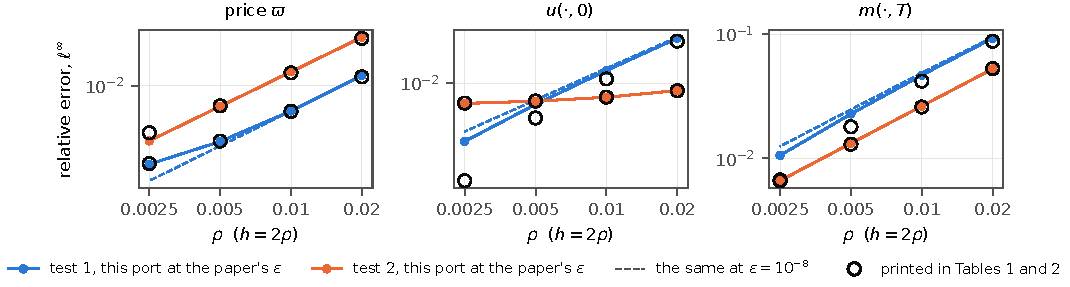
\includegraphics[width=\linewidth]{fig/mfg-redecided-agtable.pdf}
\caption{The relative errors of Table~\ref{tab:ag} against the mesh, logarithmic axes. Filled marks: this port at the paper's tolerance; dashed: the same at $\varepsilon = $ \AGTight; hollow: printed. The printed price of test 1 sits on the port's line at every mesh. The port's price errors halve as $\rho$ halves --- ratios \AGOrdersW\ (test 1) and \AGOrdersWTwo\ (test 2) at the tight tolerance --- where the printed test-1 ratios are \AGPrintedRatiosW.}
\label{fig:ag}
\end{figure}

\section{A closed form as the control (Almulla--Ferreira--Gomes)}\label{sec:afg}

\paragraph{The published object.} Almulla, Ferreira and Gomes \cite{AFG17} solve the stationary first-order game on the torus,
\[
\tfrac12 u_x^2 + V + b\,u_x = \ln m + \bar H,\qquad -\big(m(u_x + b)\big)_x = 0,\qquad \textstyle\int u = 0,\quad \int m = 1,\quad m > 0,
\]
with $V = \sin 2\pi x$, by a gradient flow and a monotone flow, and validate both against the explicit solution for $\int b = 0$ --- $u = 0$, $m = e^V/\int e^V$, $\bar H = \ln\int e^V$, their \S2.1. Of $\int b \ne 0$ they write that they are not aware of any closed-form solution; their example is $b = \cos^2 2\pi x$ (their Figures 7 and 8), $\int b = \tfrac12$, for which no table exists; the word below is \emph{enclosed}, never reproduced.

\paragraph{What was decided.} The transport equation integrates once to a constant current $j = m(u_x + b)$ --- the one-dimensional current formulation of Gomes, Nurbekyan and Prazeres \cite{GNP18}, theirs and cited --- so $u_x = j/m - b$ and the Hamilton--Jacobi equation becomes, at each $x$, the scalar equation $\ln m - j^2/(2m^2) = V - b^2/2 - \bar H$, whose left side is strictly increasing in $m$: the density is a verified inverse. Two scalars remain, fixed by $\int m = 1$ and $\int u_x = 0$, and a two-dimensional Krawczyk operator encloses them, every integral a midpoint rule with its remainder carried as an interval (\AFGKF\ cells for the map, \AFGKD\ for the Jacobian over the box); the contraction closed in \AFGRounds\ round. The same certifier run on $b = 0$ is the control: it must enclose $j$ at zero and $\bar H$ around the closed form, and it does (Table~\ref{tab:afg}); with $\int e^{\sin 2\pi x} \in \AFGIntExpVBox$ the closed form $\ln\int e^V \in \AFGCtrlCFBox$, enclosed independently, lies inside the certifier's box. For $b = \cos^2 2\pi x$ a classical solution exists with $j \in \AFGjBox$ and $\bar H \in \AFGHBox$, locally unique in that box, with the density enclosed on each of \AFGKP\ plot cells and certified above \AFGmMin, the value function enclosed with its mean removed (amplitude \AFGuAmp) and its periodicity decided ($\int u_x$ enclosed in an interval about zero of half-width \AFGClosureHalf). Global uniqueness is the paper's Lemma 2.3 and is assumed, not re-proved. The certificate carries \AFGFalsifiers\ falsifiers (the remainder deleted, the bracket's sign check disabled, the candidate moved, the closed form shifted, the floor forged), each required to refuse.

\begin{table}[t]
\centering\footnotesize\setlength{\tabcolsep}{4pt}
\caption{The first-order game of \cite{AFG17}: the control ($b = 0$, the paper's closed form) and the instance ($b = \cos^2 2\pi x$, the case without one), from the same certifier. Boxes are printed outward.}
\label{tab:afg}
\begin{tabular}{lll}
\toprule
 & $b = 0$ (the control) & $b = \cos^2 2\pi x$ (the instance) \\
\midrule
current $j$ & $\pm$\AFGCtrljHalf & \AFGjBox \\
ergodic constant $\bar H$ & \AFGCtrlHBox & \AFGHBox \\
half-widths ($j$; $\bar H$) & \AFGCtrljHalf; \AFGCtrlHHalf & \AFGjHalf; \AFGHHalf \\
density range, certified & [\AFGCtrlmMin, \AFGCtrlmMax] & [\AFGmMin, \AFGmMax] \\
closed form $\ln\int e^V$, enclosed & \AFGCtrlCFBox, inside & none known (their \S2.1) \\
verdict & \textsc{proved}; the closed form hit & \textsc{proved}: exists, locally unique, $m > 0$ \\
\bottomrule
\end{tabular}
\end{table}

\section{The effective Hamiltonian band (Gomes--Yang)}\label{sec:hbar}

\paragraph{The published object.} Gomes and Yang \cite{GY20} compute effective Hamiltonians and Mather measures by a Hessian Riemannian flow and a Newton method and test against the one case with a formula (their \S6.1, quoted from Cacace and Camilli \cite{CC16}): for $H = p^2/2 + V(x)$ on the circle, $\bar H(P) = \max V$ for $|P| \le P_0 = \int_0^1\sqrt{2(\max V - V)}$, and beyond $P_0$ the number $c$ with $\int_0^1\sqrt{2(c - V)} = |P|$; for $V = \sin 2\pi x$, $P_0 = 4/\pi$. Their Table 1 (\S6.2) is the separable two-dimensional Hamiltonian $|p|^2/2 + \cos 2\pi x_1 + \cos 2\pi x_2$ at $P = (1.5, 2.5)$, for which the paper quotes $\bar H = \HBCited$ from Gomes and Oberman \cite{GO04} beside its own flow and Newton values at $k = \HBTableOneKs$; their Table 2 (\S6.4) is $P = \HBTableTwoP$ on $-\sin 2\pi x$, where the paper states $\bar H = 1$ and reports the flow's value at $k = \HBTableTwoK$ for four meshes.

\paragraph{What was enclosed.} The formula is evaluated as intervals. $Q(c) = \int_0^1\sqrt{2(c - V)}$ is bounded by the midpoint rule with the remainder from a second-order interval jet, the cells where the base is not positive by a margin taking a Riemann bound; $c$ is bracketed by bisection on $Q$ and the bracket is closed by the mean value theorem with the period $\int 1/\sqrt{2(c - V)}$ as $Q'$. With \HBKPZero\ cells, $P_0$ is enclosed in $\HBPZeroBox$, an interval of width \HBPZeroWidth\ that contains $4/\pi = \HBFourOverPi$. On a sample of \HBSampled\ values of $P$ the band is \textsc{flat} ($\bar H = 1$ exactly) at \HBFlat\ of them, \textsc{rotating} at \HBRotating\ with brackets between \HBWidthMin\ and \HBWidthMax\ wide (\HBKSweep\ cells, the widest bracket at $P = \HBWidestP$), and \textsc{undecided} at one point, $P = 4/\pi$ itself, which lies inside the enclosure of $P_0$ (Figure~\ref{fig:hbar}).
\begingroup\sloppy
\paragraph{Their tables, held against the band.} Table 1: with \HBKTable\ cells the one-dimensional cosine values are bracketed, $c(1.5)$ in \HBCFifteenBox\ and $c(2.5)$ in \HBCTwoFiveBox, so that $\bar H(1.5, 2.5)$ lies in \HBTableOneBox, an enclosure of width \HBTableOneWidth. The quoted \HBCited\ lies \textsc{above} this enclosure by \HBCitedGap: its seventh significant digit is found not to be the value's. The paper's own values lie \textsc{below} the enclosure at every $k$, as the entropy-penalized $\bar H^k \le \bar H$ requires, and its $k = 10^4$ value \HBTableOneLastNM\ agrees with the enclosure to every digit it prints (Table~\ref{tab:hbar}). Table 2: $P = \HBTableTwoP$ is below the lower end of the $P_0$ enclosure, so the exact value is decided, $\bar H = 1$, and the printed values sit \HBTableTwoGapMin\ to \HBTableTwoGapMax\ below it, unchanged from $N = 60$ to $120$: the gap of the entropy penalization at $k = \HBTableTwoK$, not of the mesh. On the seventh digit the record says nothing about whether the quoted value is a rounding, a typo or a six-digit computation written with eight; Gomes and Oberman \cite{GO04} was not consulted, and the number is taken as \cite{GY20} prints it.\par
\endgroup

\begin{table}[t]
\centering\footnotesize
\caption{Gomes--Yang \cite{GY20}, Tables 1 and 2 held against the enclosures. Left: Table 1, $\bar H(1.5, 2.5)$, enclosure $\HBTableOneBox$; the quoted \HBCited\ is \textsc{above} it by \HBCitedGap. Right: Table 2, $P = \HBTableTwoP$ on $-\sin 2\pi x$, $k = \HBTableTwoK$.}
\label{tab:hbar}
\setlength{\tabcolsep}{4pt}
\begin{tabular}{rrlrl}
\toprule
$k$ & HRF (printed) & place & Newton (printed) & place \\
\midrule
\HBTableOneRows
\bottomrule
\end{tabular}\hspace{4mm}
\begin{tabular}{rrlr}
\toprule
$N$ & $\bar H^\diamond$ (printed) & exact $\bar H(0.5)$ & gap \\
\midrule
\HBTableTwoRows
\bottomrule
\end{tabular}
\end{table}

\begin{figure}[t]
\centering
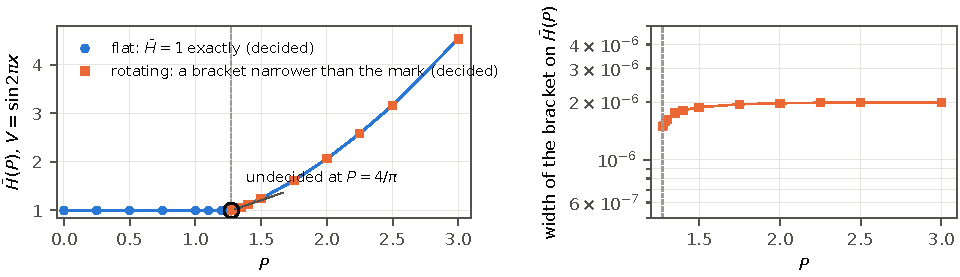
\includegraphics[width=\linewidth]{fig/mfg-redecided-hbar.pdf}
\caption{Left: the band for $V = \sin 2\pi x$ at \HBSampled\ sampled $P$ --- flat at exactly $1$ up to $P_0$, a convex rise beyond; the grey rule is the enclosure of $P_0$ (width \HBPZeroWidth) and the hollow mark the one point left undecided. Right: the width of the bracket on $\bar H(P)$ across the rotating part, between \HBWidthMin\ and \HBWidthMax, widest nearest the degeneracy.}
\label{fig:hbar}
\end{figure}

\section{The maximal value function (Gomes--\"U\c{c}er)}\label{sec:maxval}

\paragraph{The published object.} Gomes and \"U\c{c}er \cite{GU26} prove (their Theorem 1.8) that for a first-order time-dependent game with local coupling and a fixed density $m$, among all admissible subsolutions of the Hamilton--Jacobi inequality there is a unique maximal one, $u^*$, and the value functions are exactly the subsolutions equal to $u^*$ where $m > 0$ (and where $m_0 > 0$ at $t = 0$). Off the support a value function is one member of a set; the paper carries no worked example.

\paragraph{What was built and decided.} An explicit instance is built here, and said to be: on the circle of length \MVL\ with $H = \tfrac12 p^2 - m$ (their Example 2.7), a parabolic bump $m = (A(t) - B(t)x^2)_+$ of support $|x| < r(t)$ contracting under a quadratic terminal cost, with $r = 2\sin^2\theta$ and $t(\theta) = \sqrt{2/3}\,(\pi - 2\theta + \sin 2\theta)$, from $r = \MVrZero$ at $t = 0$ to $r = $ \MVrT\ at $T = \MVT \pm$ \MVTHalf, and $u = a(t)\varphi(x) + b(t)$ with $\varphi = x^2$ out to $|x| = $ \MVRhoZero\ and a $C^1$ cap beyond. On a $\MVNT \times \MVNX$ cell cylinder (\MVCells\ cells) the pair is verified on each of the \MVSupport\ support cells --- the Hamilton--Jacobi and transport residuals enclose zero --- and the strict subsolution inequality is decided on every vacuum cell by a corner bound, so $(m, u)$ is a solution in the sense of their Definition 1.1 with a vacuum, and $u$ is one member of $U(m)$. The maximal $u^*$ --- for continuous bounded $m$ the value of the control problem with running cost $\tfrac12|\dot x|^2 + m$, the classical identification \cite{BCD97}, assumed --- is enclosed on \MVDecided\ vacuum cells between the free Hopf--Lax value (a rigorous branch-and-bound over the endpoint) and the cheapest path proved clear of the moving support; on \MVTight\ of them every minimising path is proved clear and the bracket is tight; \MVRefused\ cells on the moving boundary are refused. On every decided cell $u^* \ge u$, and the gap is proved positive on \MVGapProven\ cells (\MVGapShare\% of the vacuum), reaching \MVMaxGap\ (Table~\ref{tab:maxval}). The certificate carries \MVFalsifiers\ falsifiers, among them a flipped coupling sign, a path through the crowd and a forged $u^*$.

\begin{table}[t]
\centering\footnotesize
\caption{The $\MVNT \times \MVNX$ cylinder of Section~\ref{sec:maxval}, cell by cell: the support of the contracting bump, the vacuum around it, and the seam of cells the moving boundary crosses.}
\label{tab:maxval}
\begin{tabular}{lrp{98mm}}
\toprule
standing & cells & what is decided there \\
\midrule
support & \MVSupport & $u^* = u$ by Theorem 1.8; the residuals of the pair enclose $0$ \\
vacuum, tight & \MVTight & $u^*$ equals the free Hopf--Lax value; every minimising path clear of the crowd \\
vacuum, bracket & \MVBracket & $u^*$ between the Hopf--Lax value and the cheapest path proved clear \\
refused & \MVRefused & the moving boundary crosses the cell at this budget \\
\midrule
gap $u^* - u$ proved positive & \MVGapProven & of the \MVDecided\ decided vacuum cells; the largest gap is \MVMaxGap \\
\bottomrule
\end{tabular}
\end{table}

\section{The regularization, measured (Ferreira--Gomes--\"U\c{c}er)}\label{sec:reg}

\paragraph{The published object.} Ferreira, Gomes and \"U\c{c}er \cite{FGU26} prove existence for stationary first-order games by casting the system as a monotone operator on a Banach space and adding a low-order $p$-Laplacian (their operator (3.1)) that makes it coercive; the regularization $\varepsilon$ is then sent to zero. On the one-dimensional torus with $H = |p|^2/2 - m$, a discount and $V = A\cos 2\pi x$ (their Problem 1 with power growth, $\bar\gamma = \alpha(\beta + 1)/\beta = 4$) the added terms are $\varepsilon(u'^3)'$ and $\varepsilon u^3$, polynomial; the object is the family of regularized equilibria and its limit.

\paragraph{What was proved.} Eliminating $m = u + u'^2/2 - V$ turns the transport equation into one scalar equation, $F_\varepsilon(u) = m - (m u' + \varepsilon u'^3)' + \varepsilon u^3 - 1 = 0$, whose linearization is the Sturm--Liouville operator $-(c h')' + e h$ with $c = m + (1 + 3\varepsilon)u'^2 \ge m$: elliptic wherever the density is positive, at $\varepsilon = 0$ as at $\varepsilon > 0$. A radii polynomial in the derivative-weighted space $X_2 = \{u : \sum|u_k|(1 + k)^2\nu^k < \infty\}$, $\nu = \RGNu$, with explicit columns of $I - A\,DF$ to six times the truncation and an analytic tail beyond, is asked to close a ball about a Galerkin candidate of $N = \RGNMin$ to \RGNMax\ cosine modes at every cell of a \RGCells-cell atlas, $A \in \{\RGAmpsList\}$ and $\varepsilon \in \{\RGEpsList\}$ (Figure~\ref{fig:regatlas}). \RGProved\ cells are \textsc{proved} --- a unique zero of $F_\varepsilon$ in the ball, in the even subspace, classical, with $m > 0$ on the ball, radii from \RGrMin\ to \RGrMax\ --- and \RGRefused\ are \textsc{refused} by name: \RGRefusedZOne\ with $Z_1 \ge 1$ and \RGRefusedNear\ with $Z_1$ so near $1$ that no radius closes. Along $A$ every row is proved then refused (Table~\ref{tab:regfront}): $\varepsilon = 0$ reaches $A = \RGEpsZeroLast$, $\varepsilon = \RGEpsLast$ only $A = \RGEpsLastLast$. The frontier is the certificate's, not the equation's: $Z_1$ at $\varepsilon = 0$ grows roughly linearly in $A$ as a diagonal tail inverse meets a varying coefficient $c$, while the certified density floor at the last proved cell of $\varepsilon = 0$ is \RGFloorLastZero\ and the float candidate at the first refused cell still has $\min m = \RGFloatFirstZero$.

\paragraph{What was decided.} Where a regularized cell and its unregularized neighbour are both proved (\RGDistDecided\ pairs), $\|u_\varepsilon - u_0\|_2$ is decided to a bracket of the two radii, narrower than \RGDistMaxWidth: about $\varepsilon$ at small $\varepsilon$ and sublinear beyond --- at $A = 0.4$ the ratio $\|u_\varepsilon - u_0\|_2/\varepsilon$ is \RGRatiosAFour\ for $\varepsilon = 0.01, 0.1, 0.3, 1$ --- as the constant solution already shows at $A = 0$, where $u_\varepsilon$ is the real root of $\varepsilon u^3 + u = 1$ ($u_1 = \RGuOneAtZero$, distance \RGDistZeroOne). The paper passes $\varepsilon \to 0$ by compactness; here the limit is watched on an instance, and the unregularized game certifies as far as the lightly regularized one and further than the strongly regularized ones.

\begin{table}[t]
\centering\footnotesize\setlength{\tabcolsep}{4pt}
\caption{The frontier of the atlas, per $\varepsilon$: the last amplitude proved, the first refused, the $Z_1$ that refused it, the certified density floor at the last proved cell, and the float candidate's minimum density at the first refused one.}
\label{tab:regfront}
\begin{tabular}{rrrrrr}
\toprule
$\varepsilon$ & proved to $A$ & refused from $A$ & $Z_1$ there & $m$ floor (last proved) & $\min m$ (first refused, float) \\
\midrule
\RGFrontierRows
\bottomrule
\end{tabular}
\end{table}

\begin{figure}[t]
\centering
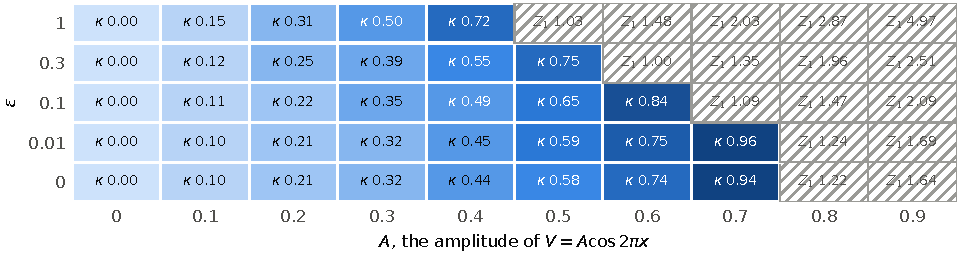
\includegraphics[width=\linewidth]{fig/mfg-redecided-regatlas.pdf}
\caption{The atlas of Section~\ref{sec:reg}: a proved cell is shaded by its contraction factor $\kappa = Z_1 + Z_2 r$ (lighter is smaller) and a refused cell is hatched with the $Z_1$ that refused it. Every row is proved then refused as $A$ grows, and the proved region shrinks as $\varepsilon$ grows.}
\label{fig:regatlas}
\end{figure}

\section{A Wardrop table (Bakaryan, Aoun, de Lima Ribeiro, Hovakimyan, Gomes)}\label{sec:wardrop}

\paragraph{The published object.} Bakaryan, Aoun, de Lima Ribeiro, Hovakimyan and Gomes \cite{BAdHG26} compute multi-population Wardrop equilibria on a network of \WDNodes\ nodes and \WDEdges\ edges by a distributed Hessian--Riemannian flow and validate each equilibrium by watching the flow settle; their Table 1 prints the edge totals of the first scenario as integers, and their Figures 2 and 4 the equilibria of the second and third.

\paragraph{What was decided.} A stopping rule cannot certify that the point it stops at is an equilibrium, that it is alone, or that its flows are positive; the three scenarios are decided again, each by the arithmetic its instance supports, in a standard-library Python verifier (\WDVerifierKB\ KB, sha256 \WDVerifierSha$\ldots$) embedded in the published reproduction page and re-run by the build of this document (Table~\ref{tab:wardrop}). S2 (cars and trucks, affine costs): the support KKT system in \WDUnknowns\ unknowns is solved over exact rationals, the Kirchhoff residual and the Wardrop gap are exactly $0$, one off-support slack is an exact tie no float tolerance could adjudicate, and the totals reproduce the published Figure 2 exactly. S3 (emission and speed--flow costs, smooth and nonlinear): an interval Krawczyk contraction proves exactly one KKT zero in a box of radius \WDBoxRadius, with support flows at least \WDFlowFloor\ and strict complementarity (every off-support slack at least \WDSlackFloor) over the box. S1 (linear cost $c = j_1 + j_2$, monotone but not strictly): the total is the exact minimum-norm optimum with Kirchhoff residual $0$ and Wardrop gap exactly $0$, and the split between the two populations is \textsc{refused}, because the split-conservation operator has an exact null space of dimension \WDNullDim\ --- the printed split is one member of a family, and no certificate of a unique split can exist. The verifier's \WDReds\ falsifiers (among them outward rounding removed, a perturbed flow, the printed Table 1 row and a wrong active set) each refuse.

\paragraph{The erratum.} Bound to the paper's Table 1, the certified S1 totals agree with the printed integers within their rounding (maximum deviation \WDMaxDevFrac\ $= \WDMaxDev$), except that the total of edge $(4, 7)$ is \WDErratumFrac\ $= \WDErratumValue$, which rounds to \WDErratumRounds\ where the table prints \WDPrinted; with the printed value, flow is not conserved at node $4$ (the falsifier shows a residual of $+2$). It is a rounding slip in a table and not a defect in the method, whose three scenarios all reproduce.

\begin{table}[t]
\centering\footnotesize\setlength{\tabcolsep}{4pt}
\caption{The three scenarios of \cite{BAdHG26}, each decided by the arithmetic its instance supports, and the one printed total found not to be what it says.}
\label{tab:wardrop}
\begin{tabular}{lp{24mm}p{33mm}p{58mm}}
\toprule
scenario & cost & instrument & verdict \\
\midrule
S1 & linear, $c = j_1 + j_2$ & exact rationals; the null space of the split-conservation operator & total \textsc{proved}, Wardrop gap exactly $0$; split \textsc{refused}: null space of dimension \WDNullDim \\
S2 & affine, cars and trucks & exact rationals, \WDUnknowns\ unknowns & \textsc{proved} exactly: Kirchhoff residual and Wardrop gap $= 0$; Figure 2 reproduced \\
S3 & emission and speed--flow, nonlinear & interval Krawczyk & \textsc{proved}: one KKT zero in a box of radius \WDBoxRadius \\
Table 1, edge $(4, 7)$ & --- & exact rationals; Kirchhoff at node $4$ & printed \WDPrinted; found to be \WDErratumFrac\ $= \WDErratumValue$ \\
\bottomrule
\end{tabular}
\end{table}

\section{The clearing price as a band (Gomes--Sa\'ude)}\label{sec:price}

\paragraph{The published object.} Gomes and Sa\'ude \cite{GS21} set the electricity price as the multiplier that makes a fleet of storage owners absorb what the grid produces, and work the linear-quadratic case with a set-point potential (their \S6): with $\Pi = \int u_x m$ and $\Xi = \int x m$ the averaged dynamics are $\dot\Xi = Q$ and $\dot\Pi = -\eta(\Xi - \kappa)$, and $\Pi$ is found through a Volterra equation and a Laplace transform up to an implicit constant; for $\eta = 0$ the price is the line $\varpi = \Theta - cQ$ with $\Theta = -\gamma(\int_0^T Q + \bar x_0 - \zeta)$, their (25) and (30).

\paragraph{What was decided.} With quadratic terminal data the other end is explicit, $\Pi(T) = \gamma(\Xi(T) - \zeta)$, and the pair integrates: $\Xi(t) = \bar x_0 + \int_0^t Q$, $\Pi(t) = \gamma(\Xi(T) - \zeta) + \eta\int_t^T(\Xi - \kappa)$, $\varpi = -cQ - \Pi$. This is three lines from the paper's own \S6.2 and is not claimed as new; what it buys is the shape: the price is affine in the supply path with every coefficient $\le 0$, so over a box $\mathrm{lo} \le Q \le \mathrm{hi}$ of supply paths the price band is attained at the corners, $\mathrm{price}(\mathrm{hi}) \le \varpi \le \mathrm{price}(\mathrm{lo})$. With $Q$ a step function on the grid and rational data every quantity is a rational number and is computed as one. On a supply scenario of $N = \PRN$ steps with $c = \PRc$, $\gamma = \PRGamma$, $\zeta = $ \PRZeta, $\bar x_0 = \PRxBar$ and the box $Q(1 \pm \rho)$, $\rho = $ \PRRhoFrac: $\Theta = $ \PRThetaExact\ $= \PRTheta$, decided as the identity $\Pi_n = -\Theta$ at all \PRGridTimes\ grid times; $\int_0^T Q = \PREnergy$ and $\Xi(T) = \PRXiT$; the band is \textsc{proved} at every grid time with both edges attained, widest at hour \PRWidestHour\ where it is \PRWidest\ (an exact rational in the record), of which \PRDayPart\ is the term $\gamma\cdot 2\rho\int_0^T Q$: \PRDayShare\% of the band at its widest is uncertainty about the day's total energy, not about the hour, whose own term never exceeds \PRInstMax; a band one price unit wide would need $\rho = \PRRhoForOne\,\%$. With a set-point preference the band is still attained at the corners; Table~\ref{tab:price} gives the ladder of $\eta$. The certificate carries \PRFalsifiers\ falsifiers, among them $\eta < 0$, where a sensitivity turns positive and a path inside the box prices outside the corner band.

\paragraph{What was measured.} A finite-difference kernel for the same system --- the implicit upwind scheme of the source laboratory the records lift from, ported bit for bit (\PRLabIt\ iterations to residual \PRLabRes\ on a $\PRLabNX \times \PRLabNT$ grid, the same price to the last bit) --- is run against the closed form. It clears the market in the agents' controls to \PRLabClearGap\ while its fleet ends the day at $\Xi(T) = \PRLabXiT$ where conservation requires \PRXiT: \PRLabLost\ of the day's \PREnergy, that is \PRLabLostPct\%, vanishes at the wall of the battery box, where the density reaches \PRWallDensityLab\ by the end of the day. Forbidding the wall-pointing control (the state-constraint wall) lowers the loss to \PRConstrainedLost; clearing on the discrete Fokker--Planck flux removes it ($\Xi(T)$ matches to \PRConsistentLost); and on the domain $[\PRWideA, \PRWideB]$, where the walls never bind, the flux-cleared scheme approaches the closed form at first order in the mesh (maximal price error \PRWideErrCoarse\ then \PRWideErrFine\ as $H$ halves, ratio \PROrder) while the lab's wall treatment does not (\PRLabWideErrCoarse\ then \PRLabWideErrFine, ratio \PRLabOrder). On the battery box the conserving scheme puts $\Pi$ at noon at \PRConsistentPiMid\ against the whole-line \PRPiZero\ --- a wall's shadow price of \PRShadow, which the lab's kernel had at \PRLabPiMid. These are floats at fixed meshes, reported as measured; what is decided is the closed form, and that only the conserving scheme measures the model.

\begin{table}[t]
\centering\footnotesize
\caption{The price band of \cite{GS21} under a $\PRRhoPct\%$ supply box, decided exactly for three set-point strengths ($\kappa = \tfrac35$ where $\eta > 0$). The width at its widest hour is split into the hour's term $c\cdot 2\rho Q(t)$, the day's term $\gamma\cdot 2\rho\int Q$ and the set-point term; $\Pi(T)$ does not see $\eta$.}
\label{tab:price}
\begin{tabular}{rrrrrrrrr}
\toprule
$\eta$ & $\kappa$ & widest band & at hour & hour's term & day's term & set-point term & $\Pi(0)$ & $\Pi(T)$ \\
\midrule
\PRLadderRows
\bottomrule
\end{tabular}
\end{table}

\section{The empty region (Alharbi--Ashrafyan--Gomes)}\label{sec:aag}

\paragraph{The published object.} Alharbi, Ashrafyan and Gomes \cite{AAG26} study first-order games on a bounded domain with an entry and an exit, and write in their abstract that contact with the exit does not necessarily imply that exit occurs. Their one-dimensional example (\S3.2) on $(0, 1)$ is $\tfrac12 u_x^2 + V = m$, $-(m u_x)_x = 0$, with inflow $-m(0)u_x(0) = j_0$, the relaxed exit $u(1) \le 0$ and the contact complementarity $u(1)\,m(1)u_x(1) = 0$, for $V = \gamma + \tfrac12\sin(3\pi(x + \tfrac14))$. Case 1 ($j_0 = 0$, $\gamma = 0$): $m = V_+$ and $u = \pm\sqrt2\int_x^1\sqrt{V_-}$, two value functions. Case 2 ($j_0 = $ \AAGjZero): $m$ is the positive root of $m^3 - Vm^2 - j_0^2/2 = 0$, positive everywhere. The figures carry no error bound, and $\gamma$ of Figure 2 is not printed.

\paragraph{What was decided.} The domain is cut into $K = \AAGK$ cells and on each the sign of $V$ is decided by an interval enclosure of the sine: \textsc{occupied} ($m = V$, enclosed), \textsc{empty} ($m = 0$ exactly) or \textsc{refused} where the enclosure straddles zero (Table~\ref{tab:aag}). The three roots are exact, $x = \tfrac1{12}, \tfrac5{12}, \tfrac34$; the certificate requires every refused cell to contain one and every root to lie in a refused cell, and the refused count is \AAGRefused\ (length $4/K = \AAGRefusedLength$) at every budget of the ladder $K = \AAGLadderKs$, from length \AAGLadderFirstLength\ down to \AAGLadderLastLength. The free boundary is not located by this --- it is exact, and the refused cells display the budget. Both value functions are enclosed by Riemann brackets from the exit, $u_+(0) \in \AAGuPlusZeroBox$ and $u_-(0)$ its negative, so the two differ by at least \AAGuGapZero\ at $x = 0$ and meet at $x = 1$, where both are exactly $0$: the value function is not unique off the support, which is their Theorem 1.3 ($Du$ unique only where $m > 0$) on an instance. The boundary conditions are evaluated as intervals: in case 1, $V(1) \in \AAGVOneBox$ so $m(1) = 0$, and $x = 1$ is in the contact set with exit flux exactly $0$ --- contact without exit, the paper's sentence decided; in case 2 the current is $-j_0$ everywhere, and the same contact carries an exit flux in $\AAGExitFluxTwoBox$. Because $\gamma$ is unprinted, case 2 is certified for every $\gamma \in \AAGGammaBox$ at once: $m \ge \AAGCaseTwoFloor$ on every cell and for every $\gamma$ in the box. The certificate carries \AAGFalsifiers\ falsifiers, the first of them the float rule that decides the sign at the cell centre and paints the root cells.

\begin{table}[t]
\centering\footnotesize
\caption{Case 1 of \cite{AAG26} on $K = \AAGK$ cells: the runs of the unit interval by standing. The refused cells hold the exact roots $\tfrac1{12}$, $\tfrac5{12}$ and $\tfrac34$; the last lies on a cell edge and takes two cells.}
\label{tab:aag}
\begin{tabular}{lll}
\toprule
run & standing & what is decided \\
\midrule
\AAGRunsRows
\bottomrule
\end{tabular}
\end{table}

\section{The shared instrument}\label{sec:method}

\paragraph{Arithmetic.} Every verdict above comes from one library, \texttt{instruments/interval} of the repository \cite{CM}: intervals over IEEE doubles with directed rounding simulated by widening every basic operation outward by one unit in the last place; the library is checked against exact BigInt rational arithmetic on random operands, with the widening removed as a control that must fail. $\exp$, $\log$, $\sin$, $\cos$ and $\tanh$ are enclosed by truncated series with rigorous remainders. Exact rational arithmetic over BigInt fractions decides what intervals cannot --- a quantity that is exactly zero, as the tie of Section~\ref{sec:wardrop} and the identities of Section~\ref{sec:price} --- and a double entered as data is converted losslessly, as $m\cdot 2^e$.

\paragraph{Integrals.} The midpoint rule with its remainder carried as an interval, $\int_{\text{cell}} f = h f(c) + E$ with $|E| \le (h^3/24)\sup_{\text{cell}}|f''|$, on $K = 2^p$ cells of $[0, 1]$ so that every node is an exact double. The bound on $f''$ comes from a second-order interval jet, the triple $(f, f', f'')$ propagated through every operation (Sections~\ref{sec:ag} and \ref{sec:hbar}); where $f''$ is unbounded, at a cusp or a zero of a root, the cell takes a plain Riemann bound and the sum stays rigorous (Sections~\ref{sec:hbar} and \ref{sec:aag}). The quadrature's own test deletes the remainder and must show the interval missing the true value on a coarse grid.

\paragraph{Contractions.} The Krawczyk operator $K(X) = x_0 - A\,F(x_0) + (I - A\,DF(X))(X - x_0)$ with strict interior containment $K(X) \subset \operatorname{int} X$ (Sections~\ref{sec:afg} and \ref{sec:wardrop}); the radii polynomial $p(r) = Y_0 - (1 - Z_1)r + \tfrac12 Z_2 r^2$ with the radius enlarged until $p(r) < 0$ holds in interval arithmetic and $\kappa = Z_1 + Z_2 r < 1$ checked as a second condition (Section~\ref{sec:reg}). The float Newton candidate and the approximate inverse $A$ are trusted for nothing.

\paragraph{The record and its falsifiers.} Each instrument writes one JSON record naming the sha256 of its code; the page that serves it re-derives the record at every build and refuses on a byte that differs. Each certificate lists its falsifiers --- planted breaks that must refuse --- and each instrument's battery fires them; a certificate that cannot go red is not accepted. The macro tool of this document re-hashes the code every record names, refuses when a record has outlived its instrument, and with \texttt{--check} re-derives all seven records in place before writing a number.

\section{Two findings, stated plainly}\label{sec:findings}

Two facts about the tables of \cite{AG25} could not be seen in the tables, and are stated plainly because a table of digits rests on them.

\paragraph{The density as printed is not one.} Both tests start from $\hat m(x) = \exp(-1/(1 - (\lambda x)^2))$ ``for $|x| < 1$, $0$ otherwise'', with $\lambda = \AGLamOne$ and $\AGLamTwo$. For $1/\lambda < |x| < 1$ the exponent $-1/(1 - (\lambda x)^2)$ is positive and unbounded as $|x| \downarrow 1/\lambda$, so the printed function has no finite integral: at $x = \AGSliverTo$ the exponent is already \AGExponentAtTo, and on the sliver $[\AGSliverFrom, \AGSliverTo]$ alone the mass is at least \AGMassOne\ for $\lambda = \AGLamOne$ (at least \AGMassTwo\ on $[\AGSliverTwoFrom, \AGSliverTwoTo]$ for $\lambda = \AGLamTwo$), decided by a one-cell Riemann bound. The only integrable reading is the standard bump with support $|x| < 1/\lambda$, which is what the paper's figures show and what Section~\ref{sec:ag} encloses, with mass $\AGMassOneBox$ and $\AGMassTwoBox$. The digits survived the re-decision, which says the authors' code used the bump and not the sentence; the sentence is found not to be a density.

\paragraph{The tolerance is inside the finest number.} The paper stops when the price moves by less than $\varepsilon = \AGEpsOne$ and reports that every case converges in \AGIterTheirs\ iterations. Run to $\varepsilon = $ \AGTight\ (\AGIterTight\ iterations) the coarse errors do not move, but at the finest mesh the price error of test 1 falls from \AGFinestTheirsW\ to \AGFinestTightW: \AGTolShare\% of the printed \AGFinestPrintedW\ is tolerance and the rest is mesh. The convergence the printed column suggests (ratios \AGPrintedRatiosW\ between its rows) is blunted at the end by $\varepsilon$ and is \AGOrdersW, clean first order, once $\varepsilon$ is out of the way. Test 2 is immune: its implicit price update reaches a residual of \AGResidTwo\ in \AGIterTwo\ iterations at every mesh, and its errors at $\varepsilon = \AGEpsTwo$ and at the tight tolerance coincide. Nothing here says a printed number is wrong; it says what the finest one is made of.

\section{What is not claimed}\label{sec:notclaimed}

Nothing in this note concerns the theorems of the eight papers: not the convergence proof of \cite{AG25}; not the uniqueness lemma of \cite{AFG17}, assumed and cited where used; not Theorem 1.8 of \cite{GU26} nor the identification of its maximal subsolution with a control value, which is classical and assumed; not the existence theory of \cite{FGU26}; not the convergence of the flow of \cite{BAdHG26}; not the existence and uniqueness of \cite{GS21}; not Theorem 1.3 of \cite{AAG26}; not the one-dimensional formula of \cite{GY20}, classical and taken as the paper cites it. What is decided is what the papers print and the objects they define on their own instances.

A \textsc{differs} cell in Table~\ref{tab:ag} is a statement about an implementation written from the paper's description with two open choices fixed; the authors' code is not published, and the choices are the likeliest reason. No reproduction of a figure is claimed: \cite{AFG17} and \cite{AAG26} print no tables, and $\gamma$ of \cite{AAG26} is unprinted and is boxed. Nothing is claimed at the undecided point $P = 4/\pi$, on a refused cell of any atlas or cylinder, outside the balls and the even subspace of Section~\ref{sec:reg}, or in two dimensions beyond the separable case of Section~\ref{sec:hbar}. The instance of Section~\ref{sec:maxval} is built here; the closed form of Section~\ref{sec:price} is not claimed as new, and the kernel measured there is the source laboratory's, not the authors'. No first anywhere is claimed: the formulas enclosed are the papers' or classical, the contraction arguments are standard \cite{Kr69,vdBL15,DLM07}, and the certified sign map with undecided cells is older than this note \cite{PV04}. The contribution is the decision grammar applied uniformly, and the public, re-runnable record.

\begingroup\sloppy
\cmrepro{The records are \texttt{certs/\allowbreak agtable-redecided.json}, \texttt{certs/\allowbreak afg-enclosure.json}, \texttt{certs/\allowbreak hbar-band.json}, \texttt{certs/\allowbreak maxval-cylinder.json}, \texttt{certs/\allowbreak regatlas.json}, \texttt{certs/\allowbreak price-band.json} and \texttt{certs/\allowbreak aag-empty-region.json}; the Wardrop verifier is \texttt{reports/\allowbreak verify\_wardrop.py}, extracted from the byte-preserved published page \texttt{legacy/\allowbreak research/\allowbreak wardrop-repro/\allowbreak wardrop-repro.html}. The instruments are \texttt{instruments/\allowbreak agtable}, \texttt{afg}, \texttt{hbar}, \texttt{maxval}, \texttt{regatlas}, \texttt{price} and \texttt{aag} on the library \texttt{instruments/\allowbreak interval}; each record is re-derived and compared byte for byte by \texttt{node instruments/<x>/run.js --check} and gated by \texttt{node instruments/<x>/battery.js}. The printed numbers of \cite{AG25} are pinned in \texttt{corpus/\allowbreak ashrafyan-gomes-2403.02785/\allowbreak tables.json}. The macros of this document are written by \texttt{node tools/\allowbreak paper-numbers/\allowbreak mfg-redecided.js [--check]}, the figures by \texttt{tools/\allowbreak paper-numbers/\allowbreak mfg-redecided-figs.py}, both from the records alone, and the document is compiled by \texttt{node tools/\allowbreak build-paper-tex.js mfg-redecided}; this build is at commit \RepoCommit.}\par
\endgroup

\footnotesize
\begin{thebibliography}{99}
\bibitem{AG25} Y.~Ashrafyan, D.~A.~Gomes, A fully-discrete semi-Lagrangian scheme for a price formation MFG model, arXiv:2403.02785v2 (30 January 2025); \S4 (the scheme), \S8 (the tests, the analytic solutions, Tables 1 and 2 on pp.~24 and 27).
\bibitem{AFG17} N.~Almulla, R.~Ferreira, D.~Gomes, Two numerical approaches to stationary mean-field games, Dynamic Games and Applications 7 (2017) 657--682, doi:10.1007/s13235-016-0203-5; arXiv:1511.06576.
\bibitem{GY20} D.~A.~Gomes, X.~Yang, The Hessian Riemannian flow and Newton's method for effective Hamiltonians and Mather measures, ESAIM: M2AN 54 (2020) 1883--1915; arXiv:1810.03483v2.
\bibitem{GU26} D.~Gomes, M.~\"U\c{c}er, Existence and structure for first-order time-dependent mean-field games with local couplings, arXiv:2606.28378 (19 June 2026).
\bibitem{FGU26} R.~Ferreira, D.~A.~Gomes, M.~\"U\c{c}er, Solving mean-field games with monotonicity methods in Banach spaces, arXiv:2506.21212v3 (2026).
\bibitem{BAdHG26} T.~Bakaryan, C.~Aoun, R.~de Lima Ribeiro, N.~Hovakimyan, D.~Gomes, Distributed Hessian--Riemannian flow for multi-population Wardrop equilibrium, AIMS Mathematics 11 (2026) 15143--15162, doi:10.3934/math.2026623.
\bibitem{GS21} D.~A.~Gomes, J.~Sa\'ude, A mean-field game approach to price formation in electricity markets, Dynamic Games and Applications 11 (2021); arXiv:1807.07088 (2018).
\bibitem{AAG26} A.~M.~Alharbi, Y.~Ashrafyan, D.~Gomes, A first-order mean-field game on a bounded domain with mixed boundary conditions, Applied Mathematics \& Optimization 93 (2026), article 40, doi:10.1007/s00245-026-10393-4; arXiv:2305.15952v4.
\bibitem{GNP18} D.~A.~Gomes, L.~Nurbekyan, M.~Prazeres, One-dimensional stationary mean-field games with local coupling, Dynamic Games and Applications 8 (2018); arXiv:1611.08161.
\bibitem{GO04} D.~A.~Gomes, A.~M.~Oberman, Computing the effective Hamiltonian using a variational approach, SIAM J.\ Control Optim.\ 43 (2004) --- as quoted in \cite{GY20}; not consulted here.
\bibitem{CC16} S.~Cacace, F.~Camilli, A generalized Newton method for homogenization of Hamilton--Jacobi equations, SIAM J.\ Sci.\ Comput.\ 38 (2016) --- as \cite{GY20} cites it.
\bibitem{Kr69} R.~Krawczyk, Newton-Algorithmen zur Bestimmung von Nullstellen mit Fehlerschranken, Computing 4 (1969) 187--201.
\bibitem{vdBL15} J.~B.~van den Berg, J.-P.~Lessard, Rigorous numerics in dynamics, Notices Amer.\ Math.\ Soc.\ 62 (2015).
\bibitem{DLM07} S.~Day, J.-P.~Lessard, K.~Mischaikow, SIAM J.\ Numer.\ Anal.\ 45 (2007) --- the radii polynomial, as the record's page \texttt{reports/regatlas.html} cites it.
\bibitem{BCD97} M.~Bardi, I.~Capuzzo-Dolcetta, Optimal Control and Viscosity Solutions of Hamilton--Jacobi--Bellman Equations, Birkh\"auser, 1997.
\bibitem{PV04} S.~Plantinga, G.~Vegter, Isotopic approximation of implicit curves and surfaces, Symposium on Geometry Processing (2004) --- the certified sign map, as the record's page \texttt{reports/aag.html} cites it.
\bibitem{CM} C.~Toledo, cert-machine: independent exact certification of machine-generated mathematics, \url{https://github.com/carlostoledo1891/cert-machine}, commit \RepoCommit.
\end{thebibliography}

\end{document}
